\capitulo{5}{Aspectos relevantes del desarrollo del proyecto}


En este apartado se detallarán los aspectos más relevantes del proyecto.

\section{Motivación en la elección del proyecto}

La motivación a la hora de elegir este proyecto surgió por lo interesante de la premisa, tratar con datos de sensores reales y diseñar un sistema que no solo mantenga monitorizados dichos sensores, sino que aprenda de ellos resulto ser suficiente para la elección de este proyecto. 

\section{Desarrollo del proyecto}

\subsection{Inicio}

Las primeras semanas tras la asignación del proyecto se destinaron en asentar la idea general del proyecto y a establecer una serie de objetivos, así como la ruta que había que llevar para lograrlos con éxito.

Durante esta primera etapa, la mayoría del tiempo se destinó al aprendizaje y a la investigación de posibles herramientas y tecnologías que podrían ser de utilidad.

Se eligió Elasticsearch como principal motor de búsqueda y como base de datos para los sensores. A partir de ahí comenzó el desarrollo del proyecto.

\subsection{Reuniones con el cliente}

A lo largo del proyecto se celebraron una serie de reuniones con el cliente, el cual dispone de una serie de sensores encargados de medir ciertos parámetros de una bodega. Estos sensores los tenía conectados al software de monitorización PRTG, por lo tanto, se estableció como punto de partida y cómo uno de los primeros objetivos el recopilar los datos de PRTG. 

\subsection{Conexión entre servidores}
El primer gran reto que se presentó fue realizar la conexión entre el servidor PRTG con los sensores del cliente configurados y el servidor Ubuntu, el cual contiene Elasticsearch que se encargaría de la monitorización de dichos sensores. 

A la hora de descargar los datos de PRTG surgieron una serie de adversidades que se fueron solucionando, estos inconvenientes se encuentran detallados en el apartado \ref{cap:Problemas}. Una vez se logró que se fueran descargando los datos procedentes de PRTG de forma periódica llego la hora de configurar las herramientas de \textit{ELK Stack} para poder tratar los datos obtenidos y poder indexarlos correctamente en Elasticsearch.

Una vez conseguida la conexión entre los dos sistemas y logrado un flujo continuo de datos también se logró uno de los objetivos propuestos, monitorizar los datos. Gracias a Elasticsearch y Kibana se podía mantener un control sobre los datos de los sensores pudiendo representarlo de diversas formas gráficas.

\subsection{Aplicación de modelos machine learning}

El siguiente gran reto fue la realización de un modelo capaz de poder aprender de los datos recibidos y así poder realizar predicciones a futuro.

Durante esta etapa se llevó a cabo la investigación sobre que métodos y algoritmos utilizar. Se llegó a la conclusión de que la mejor idea y la más interesante, sería implementar algoritmos de aprendizaje incremental, de esta forma el modelo que se cree podrá aprender según obtenga los datos. Para ello se decidió la utilización de la librería de Python River, la cual, pese a seguir en desarrollo y contar con una documentación aún por terminar, es una librería prometedora.

Se diseñó un sistema con el cual tras descargarse de los datos de PRTG y almacenarlos en Elasticsearch se volvían a extraer para poder ser entrenados por un modelo. Se decidió que se almacenaran y luego se volvieran a extraer en vez de utilizar los datos obtenidos directamente de PRTG porque de esta forma el entrenamiento no dependía de PRTG y si se desactiva esta funcionalidad durante un tiempo y se vuelve a activar después, poder tener la opción de entrenar el modelo con datos pasados.

\begin{figure}[h]
	\centering
	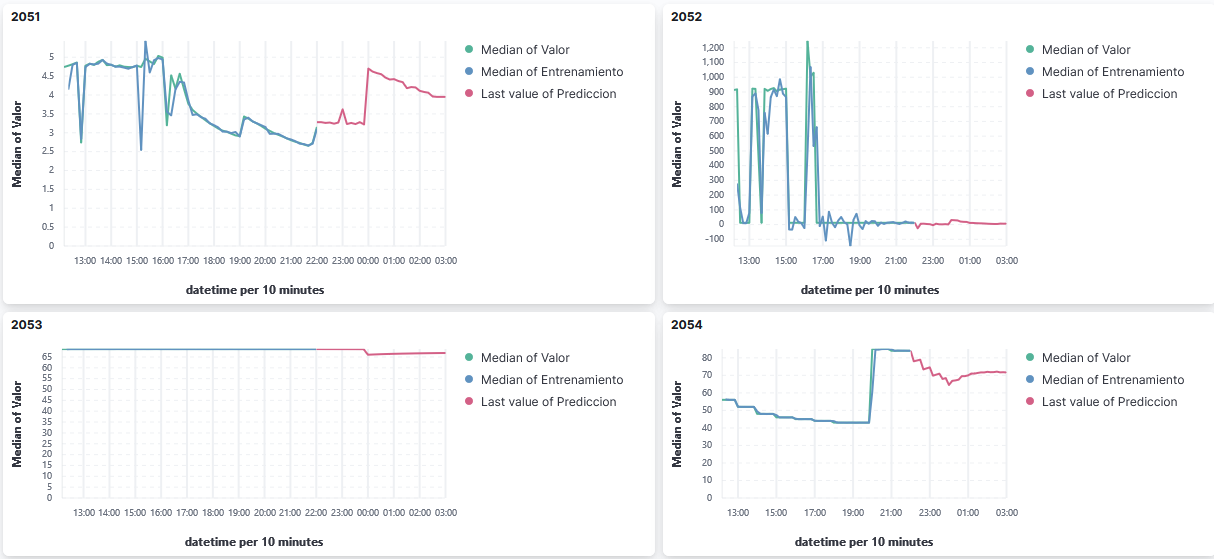
\includegraphics[width=1.1\textwidth]{img/img_monitorizacion_sensores.png}
	\caption{monitorización de sensores}
	\label{img_monitorizacion_sensores}
\end{figure}

\subsection{Pruebas y resultados}

Tras realizar las pruebas sobre los modelos se llegó a una desilusionante conclusión y es que sus predicciones no eran lo suficientemente buenas.

Debido a la poca experiencia y conocimientos en este campo no se pudo optimizar los modelos para que hicieran predicciones aceptables.

\subsection{Facilitar la instalación}
Para terminar, debido a la compleja configuración de todos los sistemas involucrados se decidió realizar un instalador que facilitará al usuario poner en marcha el programa.

\section{Problemas y resoluciones}\label{cap:Problemas}
A continuación, se mostrarán una serie de problemas que se fueron presentando durante todo el desarrollo del proyecto, así como la solución a la que se llegó.

\begin{itemize}
    \item El primer inconveniente que se presento fue a la hora de descargar los datos de PRTG ya que no permite descargar datos en intervalos menores a media hora. Para solucionar este problema y poder descargar los datos de forma más continua, se decidió descargar desde PRTG en intervalos de media hora pero realizar esta acción con una periodicidad de un minuto, de esta forma la primera vez que se ejecuta el programa se suben los datos descargados en su totalidad pero en los ciclos posteriores el nuevo conjunto de datos descargados de PRTG (con un rango de media hora) es comparado con el del ciclo anterior eliminando los datos repetidos, de esta forma se logra sacar los datos correspondientes al último minuto.
    
    
    \item Al descargarse los datos desde PRTG estos se encontraban con un formato difícil de procesar por logstash (ya que este está pensado principalmente para trabajar con logs). Por ello se decidió realizar un sencillo programa en flex que transformara las líneas de datos en un formato legible para logstash.
    
    Tras unos meses, se vio necesario realizar un tratamiento del campo fecha, La horas descargadas por PRTG vienen en un formato H:mm:ss mientras que Logstash lee las horas con un formato HH:mm:ss por lo que al encontrarse horas de un solo dígito logstash no lo reconocía y saltaba una excepción.
    
    se utilizó flex en un primer lugar por su sencillez, pero tras esta nueva necesidad se vio necesario migrar esta funcionalidad a Python y prescindir del programa realizado en flex.
    
    \item Elasticsearch almacena las variables de tiempo en formato UTC pero a la ahora de visualizar los datos en kibana se utiliza por defecto la zona horaria del navegador.
    
    Una forma de solucionarlo es configurar Kibana para que cambiar la zona horaria a UTC.
    
    \item PRTG solo recoge los datos de los sensores cuando este se encuentre en un equipo encendido y con acceso a internet, si no, los datos procedentes de los sensores se pierden, haciendo que nunca se guardarán datos de varios días seguidos.
    
    Para solucionar esto se debería migrar el sistema a un servidor que se mantenga funcional siempre.
\end{itemize}
